\documentclass{standalone}
\usepackage{tikz}
\usetikzlibrary{patterns, positioning}


\begin{document}
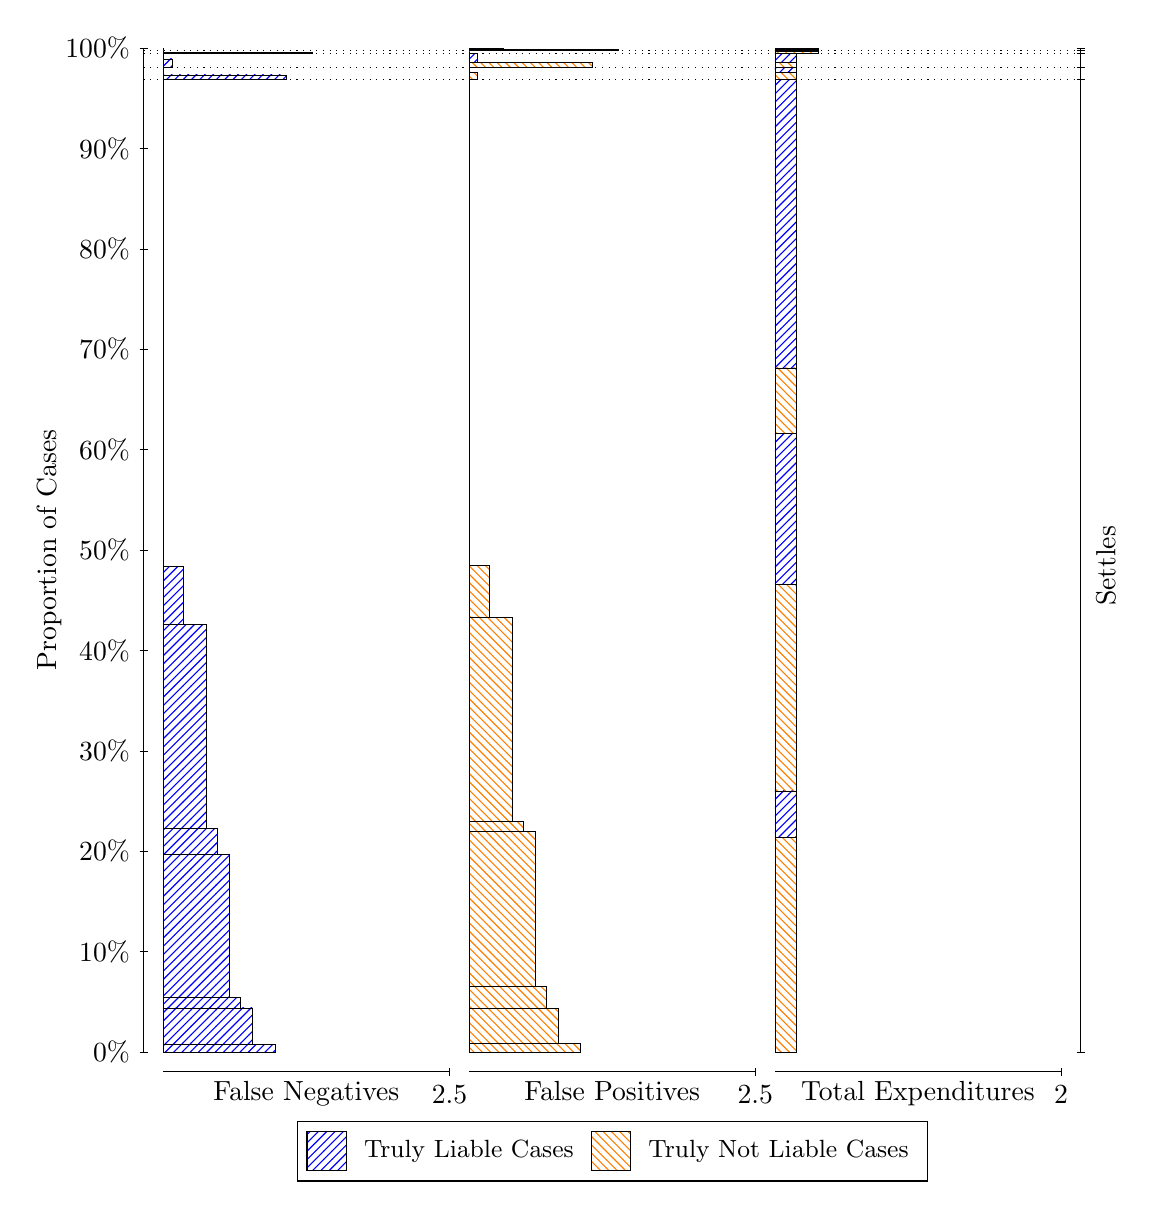
\begin{tikzpicture}
\draw[black, very thin] (1.5,1.75) -- (1.5,14.5);
\node[rotate=90, text=black, anchor=center] at (0.3, 8.125) {Proportion of Cases};
\draw[black, very thin] (1.45,1.75) -- (1.55,1.75);
\node[text=black, anchor=east] at (1.45, 1.75) {0\%};
\draw[black, very thin] (1.45,3.025) -- (1.55,3.025);
\node[text=black, anchor=east] at (1.45, 3.025) {10\%};
\draw[black, very thin] (1.45,4.3) -- (1.55,4.3);
\node[text=black, anchor=east] at (1.45, 4.3) {20\%};
\draw[black, very thin] (1.45,5.575) -- (1.55,5.575);
\node[text=black, anchor=east] at (1.45, 5.575) {30\%};
\draw[black, very thin] (1.45,6.85) -- (1.55,6.85);
\node[text=black, anchor=east] at (1.45, 6.85) {40\%};
\draw[black, very thin] (1.45,8.125) -- (1.55,8.125);
\node[text=black, anchor=east] at (1.45, 8.125) {50\%};
\draw[black, very thin] (1.45,9.4) -- (1.55,9.4);
\node[text=black, anchor=east] at (1.45, 9.4) {60\%};
\draw[black, very thin] (1.45,10.675) -- (1.55,10.675);
\node[text=black, anchor=east] at (1.45, 10.675) {70\%};
\draw[black, very thin] (1.45,11.95) -- (1.55,11.95);
\node[text=black, anchor=east] at (1.45, 11.95) {80\%};
\draw[black, very thin] (1.45,13.225) -- (1.55,13.225);
\node[text=black, anchor=east] at (1.45, 13.225) {90\%};
\draw[black, very thin] (1.45,14.5) -- (1.55,14.5);
\node[text=black, anchor=east] at (1.45, 14.5) {100\%};

\draw[black, very thin] (13.4,1.75) -- (13.4,14.5);
\draw[black, very thin] (13.35,1.75) -- (13.45,1.75);
\node[anchor=west] at (13.35, 1.75) {};
\draw[black, very thin] (13.35,14.097) -- (13.45,14.097);
\node[anchor=west] at (13.35, 14.097) {};
\draw[black, very thin] (13.35,14.252) -- (13.45,14.252);
\node[anchor=west] at (13.35, 14.252) {};
\draw[black, very thin] (13.35,14.432) -- (13.45,14.432);
\node[anchor=west] at (13.35, 14.432) {};
\draw[black, very thin] (13.35,14.466) -- (13.45,14.466);
\node[anchor=west] at (13.35, 14.466) {};
\draw[black, very thin] (13.35,14.5) -- (13.45,14.5);
\node[anchor=west] at (13.35, 14.5) {};

\draw[black, very thin, pattern color=blue, pattern=north east lines] (1.75,1.75) rectangle (3.167,1.851);
\draw[black, very thin, pattern color=blue, pattern=north east lines] (1.75,1.851) rectangle (2.8763,2.3103);
\draw[black, very thin, pattern color=blue, pattern=north east lines] (1.75,2.3103) rectangle (2.731,2.4437);
\draw[black, very thin, pattern color=blue, pattern=north east lines] (1.75,2.4437) rectangle (2.5857,4.2603);
\draw[black, very thin, pattern color=blue, pattern=north east lines] (1.75,4.2603) rectangle (2.4403,4.5944);
\draw[black, very thin, pattern color=blue, pattern=north east lines] (1.75,4.5944) rectangle (2.295,7.184);
\draw[black, very thin, pattern color=blue, pattern=north east lines] (1.75,7.184) rectangle (2.0043,7.9182);
\draw[black, very thin, pattern color=orange, pattern=north west lines] (1.75,7.9182) rectangle (1.75,14.097);
\draw[black, very thin, pattern color=blue, pattern=north east lines] (1.75,14.097) rectangle (3.3123,14.16);
\draw[black, very thin, pattern color=orange, pattern=north west lines] (1.75,14.16) rectangle (1.75,14.252);
\draw[black, very thin, pattern color=blue, pattern=north east lines] (1.75,14.252) rectangle (1.859,14.363);
\draw[black, very thin, pattern color=orange, pattern=north west lines] (1.75,14.363) rectangle (1.75,14.432);
\draw[black, very thin, pattern color=blue, pattern=north east lines] (1.75,14.432) rectangle (3.6393,14.443);
\draw[black, very thin, pattern color=orange, pattern=north west lines] (1.75,14.443) rectangle (1.75,14.466);
\draw[black, very thin, pattern color=orange, pattern=north west lines] (1.75,14.466) rectangle (1.75,14.478);
\draw[black, very thin, pattern color=blue, pattern=north east lines] (1.75,14.478) rectangle (1.75,14.5);
\draw[black, very thin, pattern color=orange, pattern=north west lines] (5.6333,1.75) rectangle (7.0503,1.8575);
\draw[black, very thin, pattern color=orange, pattern=north west lines] (5.6333,1.8575) rectangle (6.7597,2.2998);
\draw[black, very thin, pattern color=orange, pattern=north west lines] (5.6333,2.2998) rectangle (6.6143,2.5814);
\draw[black, very thin, pattern color=orange, pattern=north west lines] (5.6333,2.5814) rectangle (6.469,4.5481);
\draw[black, very thin, pattern color=orange, pattern=north west lines] (5.6333,4.5481) rectangle (6.3237,4.6815);
\draw[black, very thin, pattern color=orange, pattern=north west lines] (5.6333,4.6815) rectangle (6.1783,7.271);
\draw[black, very thin, pattern color=orange, pattern=north west lines] (5.6333,7.271) rectangle (5.8877,7.929);
\draw[black, very thin, pattern color=blue, pattern=north east lines] (5.6333,7.929) rectangle (5.6333,14.097);
\draw[black, very thin, pattern color=orange, pattern=north west lines] (5.6333,14.097) rectangle (5.7423,14.19);
\draw[black, very thin, pattern color=blue, pattern=north east lines] (5.6333,14.19) rectangle (5.6333,14.252);
\draw[black, very thin, pattern color=orange, pattern=north west lines] (5.6333,14.252) rectangle (7.1957,14.321);
\draw[black, very thin, pattern color=blue, pattern=north east lines] (5.6333,14.321) rectangle (5.7423,14.432);
\draw[black, very thin, pattern color=orange, pattern=north west lines] (5.6333,14.432) rectangle (5.6333,14.455);
\draw[black, very thin, pattern color=blue, pattern=north east lines] (5.6333,14.455) rectangle (5.6333,14.466);
\draw[black, very thin, pattern color=orange, pattern=north west lines] (5.6333,14.466) rectangle (7.5227,14.478);
\draw[black, very thin, pattern color=blue, pattern=north east lines] (5.6333,14.478) rectangle (6.0693,14.5);
\draw[black, very thin, pattern color=orange, pattern=north west lines] (9.5167,1.75) rectangle (9.7892,4.4728);
\draw[black, very thin, pattern color=blue, pattern=north east lines] (9.5167,4.4728) rectangle (9.7892,5.0655);
\draw[black, very thin, pattern color=orange, pattern=north west lines] (9.5167,5.0655) rectangle (9.7892,7.6903);
\draw[black, very thin, pattern color=blue, pattern=north east lines] (9.5167,7.6903) rectangle (9.7892,9.6079);
\draw[black, very thin, pattern color=orange, pattern=north west lines] (9.5167,9.6079) rectangle (9.7892,10.439);
\draw[black, very thin, pattern color=blue, pattern=north east lines] (9.5167,10.439) rectangle (9.7892,14.097);
\draw[black, very thin, pattern color=orange, pattern=north west lines] (9.5167,14.097) rectangle (9.7892,14.19);
\draw[black, very thin, pattern color=blue, pattern=north east lines] (9.5167,14.19) rectangle (9.7892,14.252);
\draw[black, very thin, pattern color=orange, pattern=north west lines] (9.5167,14.252) rectangle (9.7892,14.321);
\draw[black, very thin, pattern color=blue, pattern=north east lines] (9.5167,14.321) rectangle (9.7892,14.432);
\draw[black, very thin, pattern color=orange, pattern=north west lines] (9.5167,14.432) rectangle (10.062,14.455);
\draw[black, very thin, pattern color=blue, pattern=north east lines] (9.5167,14.455) rectangle (10.062,14.466);
\draw[black, very thin, pattern color=orange, pattern=north west lines] (9.5167,14.466) rectangle (10.062,14.478);
\draw[black, very thin, pattern color=blue, pattern=north east lines] (9.5167,14.478) rectangle (10.062,14.5);
\draw[black, dotted] (1.5,14.097) -- (13.4,14.097);
\draw[black, dotted] (1.5,14.252) -- (13.4,14.252);
\draw[black, dotted] (1.5,14.432) -- (13.4,14.432);
\draw[black, dotted] (1.5,14.466) -- (13.4,14.466);
\draw[black, very thin] (1.75,1.5) -- (5.3833,1.5);
\node[text=black, anchor=north] at (3.5667, 1.5) {False Negatives};
\draw[black, very thin] (5.3833,1.45) -- (5.3833,1.55);
\node[text=black, anchor=north] at (5.3833, 1.45) {2.5};

\draw[black, very thin] (5.6333,1.5) -- (9.2667,1.5);
\node[text=black, anchor=north] at (7.45, 1.5) {False Positives};
\draw[black, very thin] (9.2667,1.45) -- (9.2667,1.55);
\node[text=black, anchor=north] at (9.2667, 1.45) {2.5};

\draw[black, very thin] (9.5167,1.5) -- (13.15,1.5);
\node[text=black, anchor=north] at (11.333, 1.5) {Total Expenditures};
\draw[black, very thin] (13.15,1.45) -- (13.15,1.55);
\node[text=black, anchor=north] at (13.15, 1.45) {2};

\node[text=black, centered, rotate=90] at (13.72, 7.9236) {Settles};





\draw (7.449999999999999,1.5) node[draw=none] (baseCoordinate) {};
\begin{scope}[align=center]
        \matrix[scale=0.5, draw=black, below=0.5cm of baseCoordinate, nodes={draw}, column sep=0.1cm]{
            \node[rectangle, draw, minimum width=0.5cm, minimum height=0.5cm, pattern color=blue, pattern=north east lines] {}; &
            \node[draw=none, font=\small, text=black] (B) {Truly Liable Cases}; &
            \node[rectangle, draw, minimum width=0.5cm, minimum height=0.5cm, pattern color=orange, pattern=north west lines] {}; &
            \node[draw=none, font=\small, text=black] (B) {Truly Not Liable Cases}; \\
            };
\end{scope}

\end{tikzpicture}
\end{document}